\documentclass[9pt]{article}

\usepackage{amssymb}
\usepackage{amsmath}
\usepackage{amsfonts}
\usepackage{comment}
\usepackage{fancyhdr}
\usepackage{mathrsfs}
\usepackage{enumitem}
\usepackage{graphicx}

\usepackage{tikz}

\voffset = -50pt
%\textheight = 700pt
\addtolength{\textwidth}{60pt}
\addtolength{\evensidemargin}{-30pt}
\addtolength{\oddsidemargin}{-30pt}
%\setlength{\headheight}{44pt}

\newcommand{\qed}{\hfill \ensuremath{\Box}}


\newcommand*\circled[1]{\tikz[baseline=(char.base)]{
            \node[shape=circle,draw,inner sep=2pt] (char) {#1};}}

\newcommand{\Z}{\mathbb{Z}}
\newcommand{\I}{\mathbb{I}}
\newcommand{\M}{\mathbb{M}}
\newcommand{\R}{\mathbb{R}}
\newcommand{\C}{\mathbb{C}}
%\setcounter{section}{-1}

\begin{document}
\topskip0pt
\vspace*{\fill}
\begin{center}
{\Huge \begin{tabular}{@{}ll@{}}
   Class: & CECS 201, Section 7 \\ \\ \\
   Lab: & 10 \\ \\ \\
   Title: & Digital Clock \\ \\ \\
   Student Name: & Barry Joseph Okonoboh \\ \\ \\
   Due Date: & 11:59:59 P.M., 06, May 2015 \\ \\ \\
   Instructor: & Dan Cregg
\end{tabular}}
\end{center}
\vspace*{\fill}
\newpage
\begin{enumerate}
%%%%%%%%%%%%%%%%%%%%%%%%%%%%%%%%%%%%%%%%01%%%%%%%%%%%%%%%%%%%%%%%%%%%%%%%%%%%%%%
   \item[\textbf{Introduction.}]  In this lab, the student is tasked with 
   creating a digital clock using all the tools that he has learned during the
   course of the semester.
   
   \item[\textbf{Description.}] Our digital clock will use the leftmost
   7-segment LEDs to display the hour (ranging from 00-23), the two 
   rightmost LEDs to display the minute(ranging from 00-59), and the
   6 rightmost green LEDs (N11,M11,V15,U15,V16,U16) to display the seconds.   
   The 7-segment LEDs will display their data in decimal while the green LEDs
   will display their data in binary (U16 is the least significant bit). \\
   
   T5 will be used to enable or disable clock and C9 will be used to set the
   clock. \\
   
   In building this clock we shall be using a myriad of building blocks, and
   they are described below:
  	\item[\textbf{SecondsCounter.}] \textbf{Schematic.}
   
             \begin{center}
                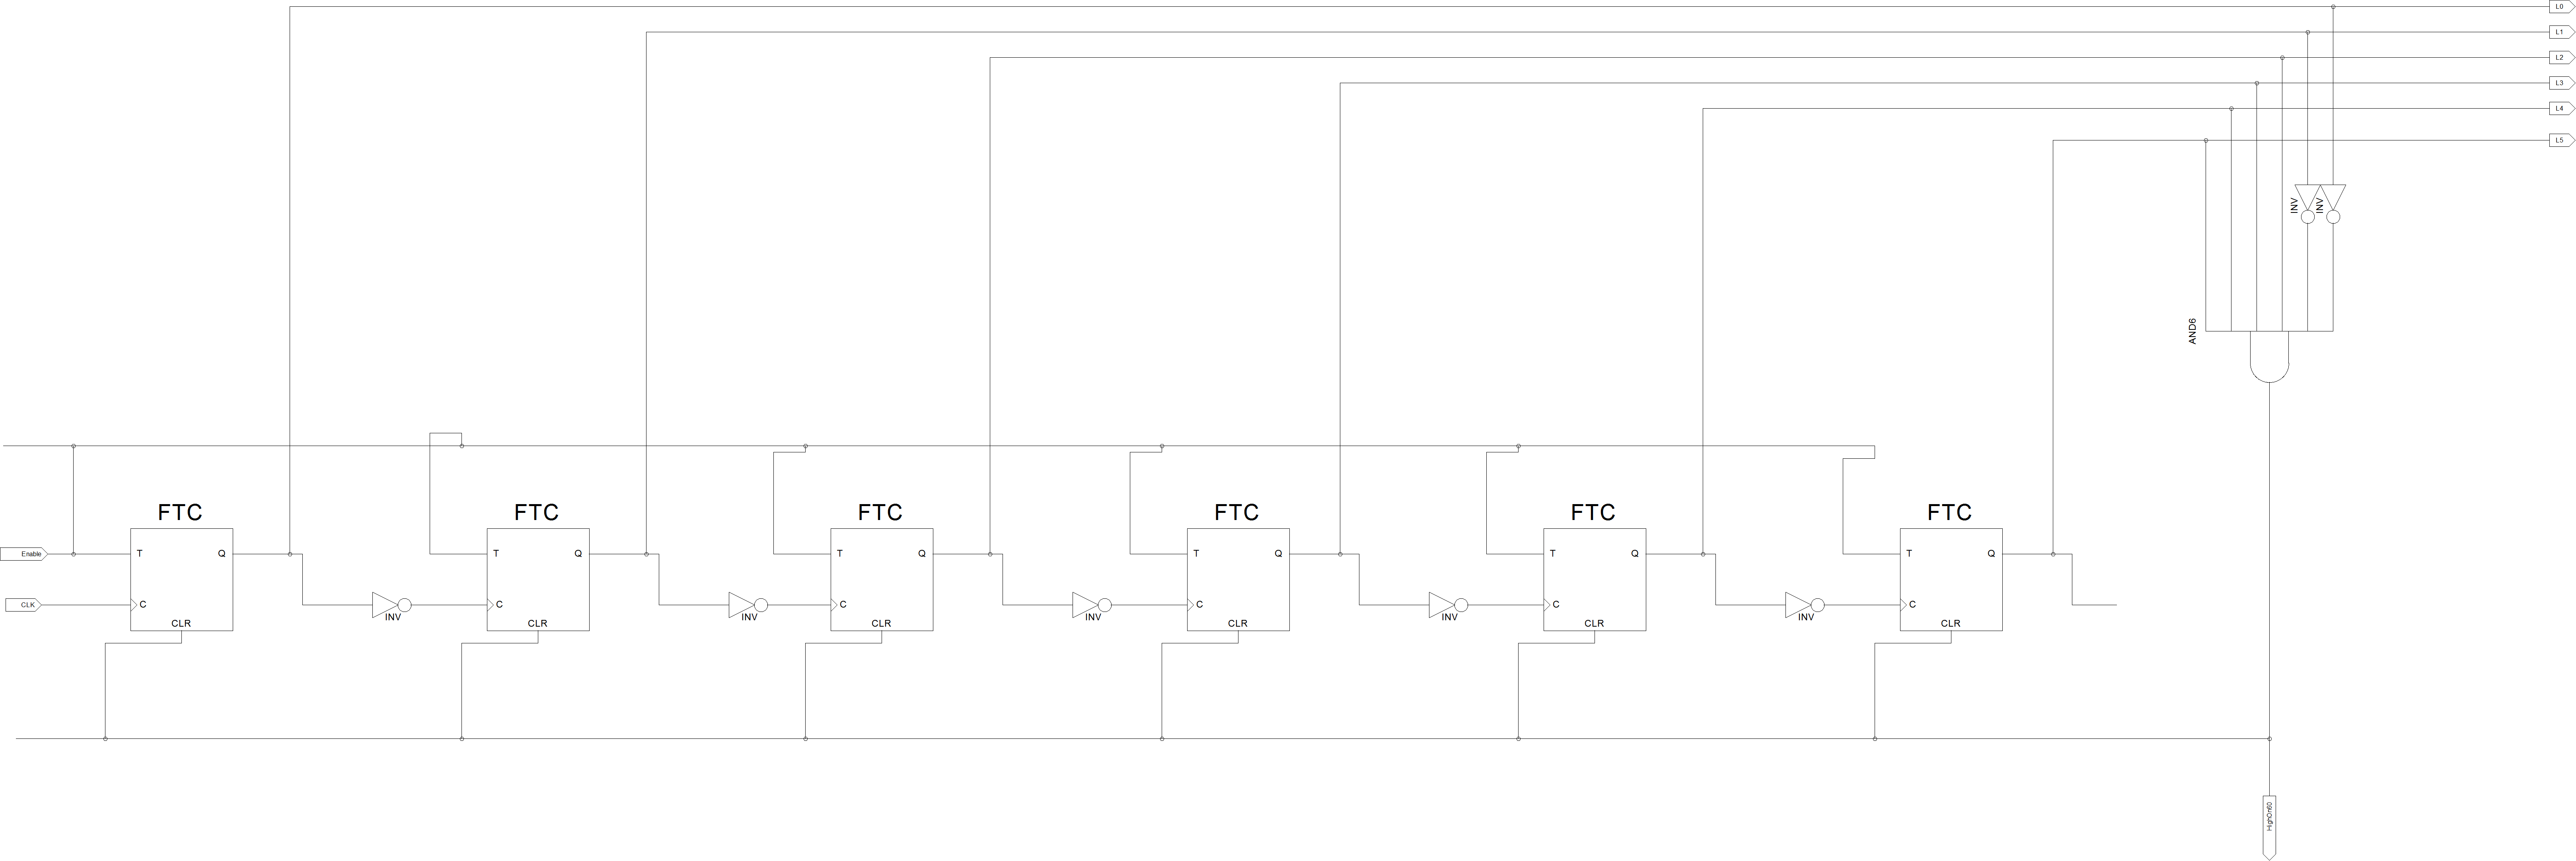
\includegraphics[width=\textwidth]{seconds_counter.png}
             \end{center}
             
             \newpage
             \textbf{Symbol.}
   
             \begin{center}
                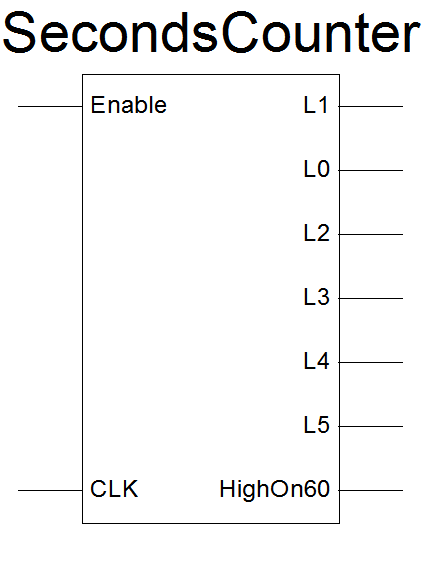
\includegraphics[width=\textwidth]{seconds_counter_sym.png}
             \end{center}
             
             \textbf{Description.} The seconds counter is a 2-input to 7-output
             counter. It counts from 0 - 59 and resets on 60. On each clock
             input, it increments by 1, and its current states are stored in
             the outputs L5, L4, L3, L2, L1, and L0, listed from most significant
             bit to least significant bit. When the state is momentarily
             $111100_2$ ($60_{10}$), the output HighOn60 goes high. We shall be
             using this circuit to count the seconds by tying the outputs to
             the appropriate locations ((N11,M11,V15,U15,V16,U16) on the board.
             
  	\item[\textbf{DecadeCounterPlus.}] \textbf{Schematic.}
   
             \begin{center}
                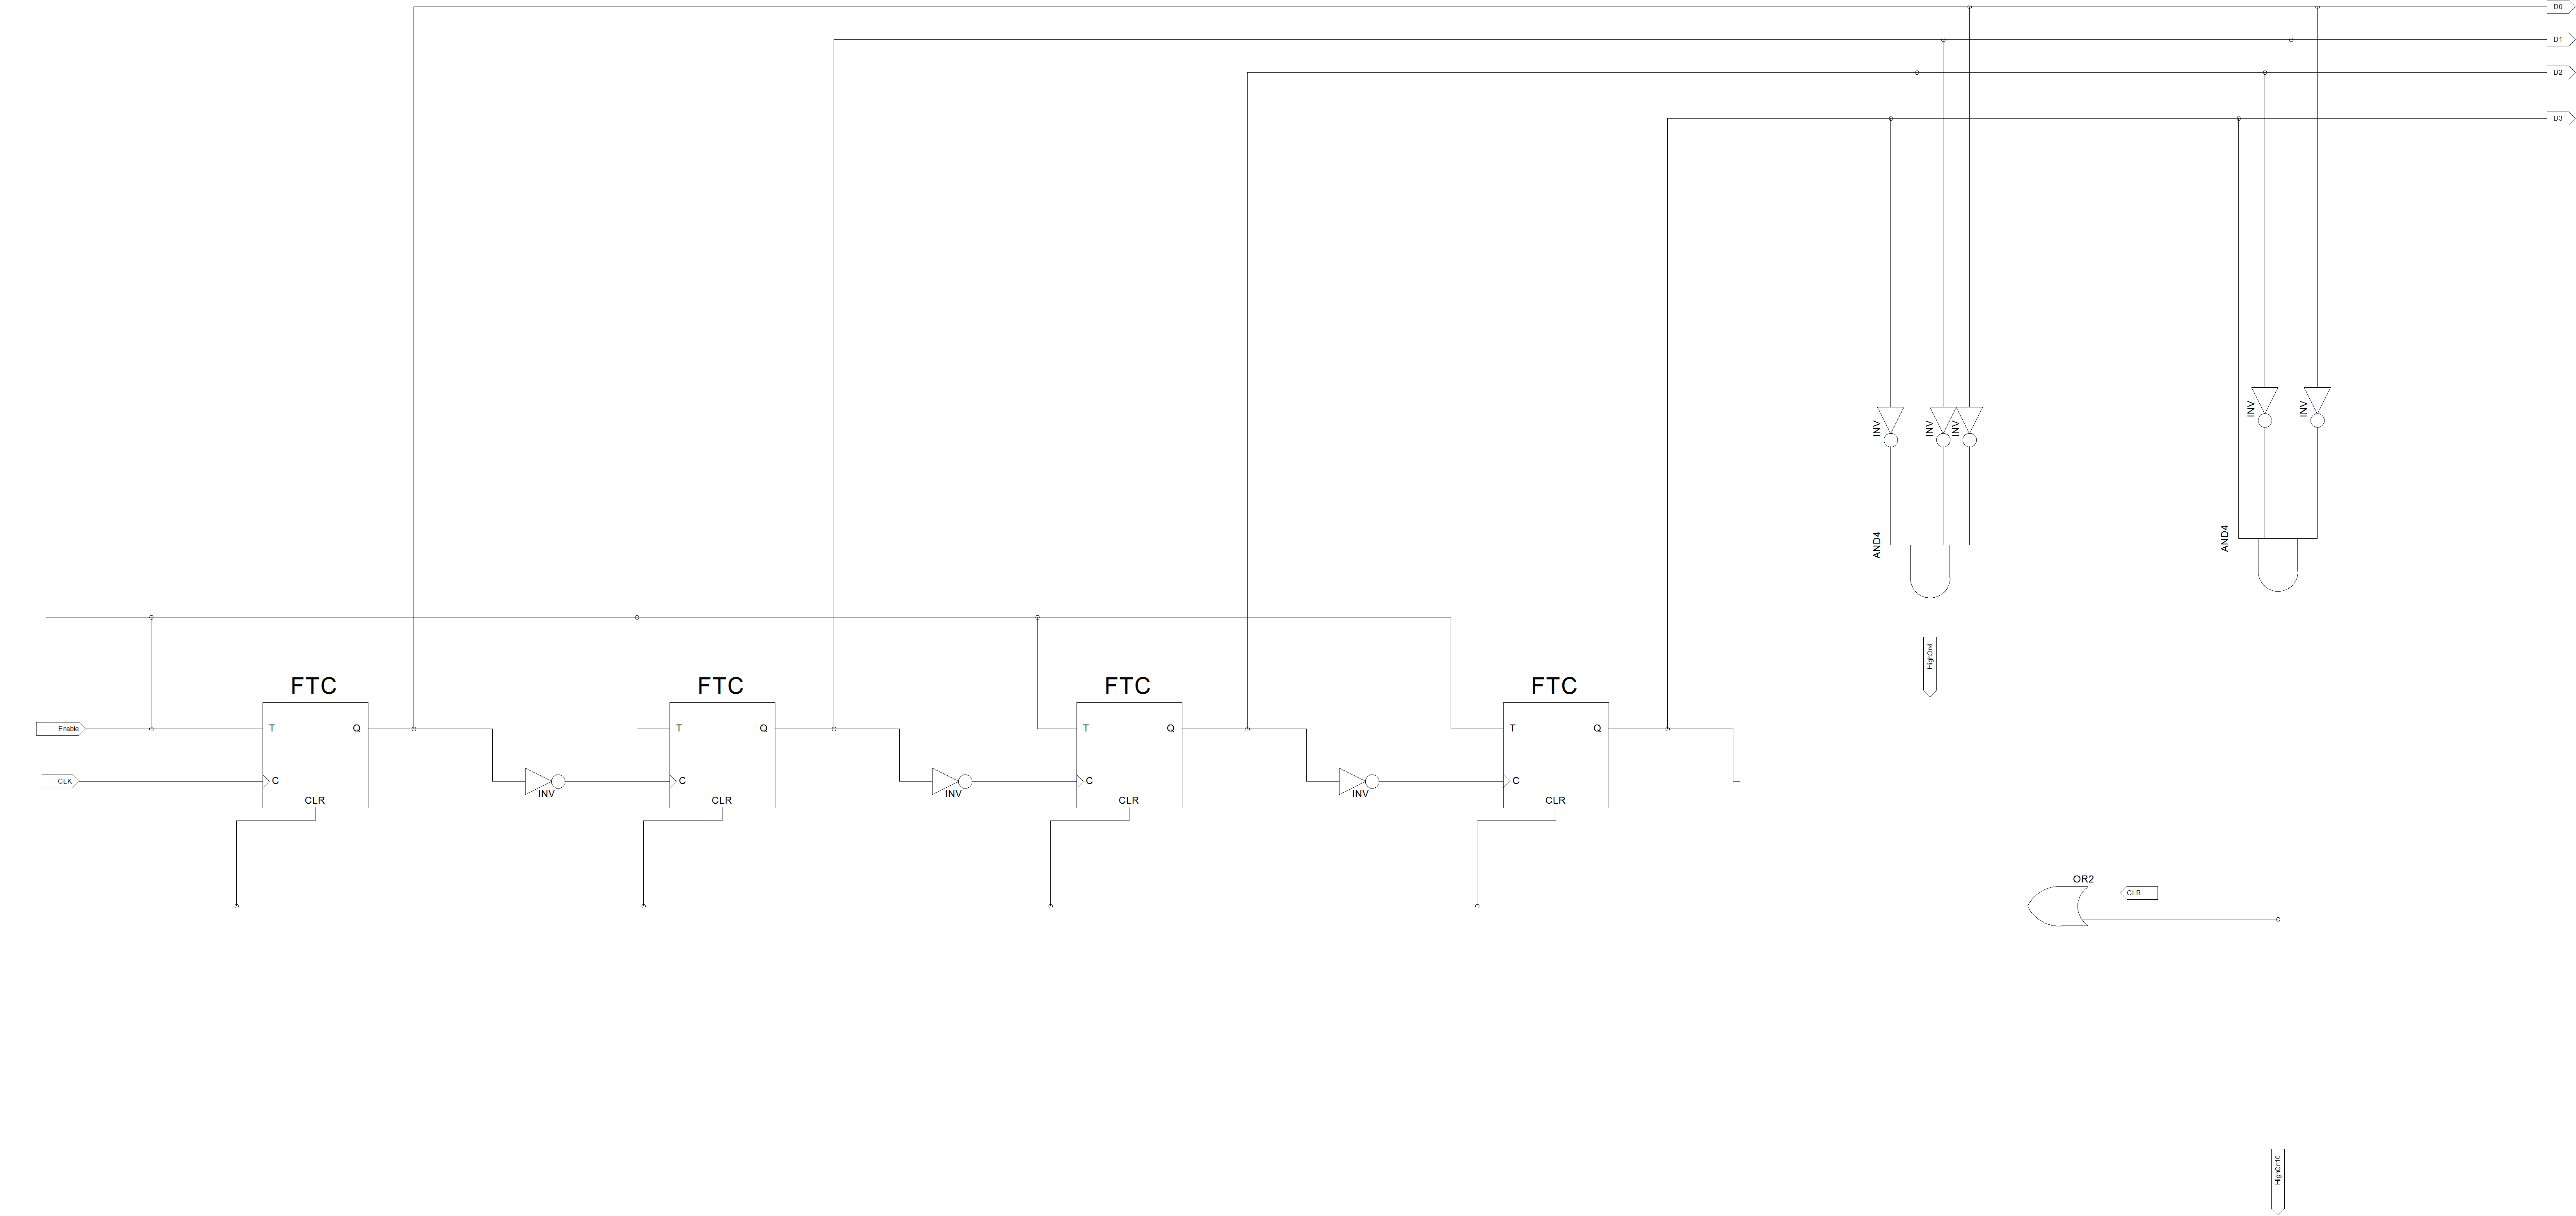
\includegraphics[width=\textwidth]{decade_counter_plus.png}
             \end{center}
             
             \newpage
             \textbf{Symbol.}
   
             \begin{center}
                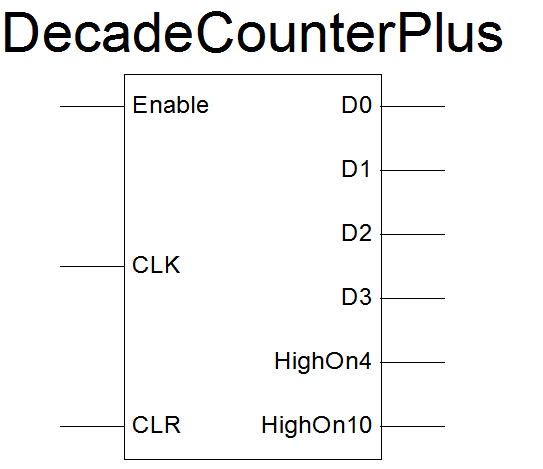
\includegraphics[width=\textwidth]{decade_counter_plus_sym.png}
             \end{center}
             
             \textbf{Description.} The decade counter plus is a 3-input to
             6-output counter. It counts from 0 - 9 and resets on 10. On each
             clock input, it increments by 1, and its current states are stored in
             the outputs D3, D2, D1, and D0, listed from most significant
             bit to least significant bit. When the state is momentarily
             $1010_2$ ($10_{10}$), the output HighOn10 goes high; similarly
             when the state is momentarily $0100_2$ ($4_{10}$), the output
             HighOn4 goes high. Why do we need the HighOn4 output? We need it
             because we shall be using this circuit for both the minute ones
             and the hours ones. For the minute ones, we do not need the
             HighOn4 output; however, we need it for the hours ones because
             we need to know when the hour segment is at 09 and at 23. For the
             former we transition from 09 to 10, and for the latter we
             transition from 23 to 00.
             
  	\item[\textbf{Minute6Counter.}] \textbf{Schematic.}
   
             \begin{center}
                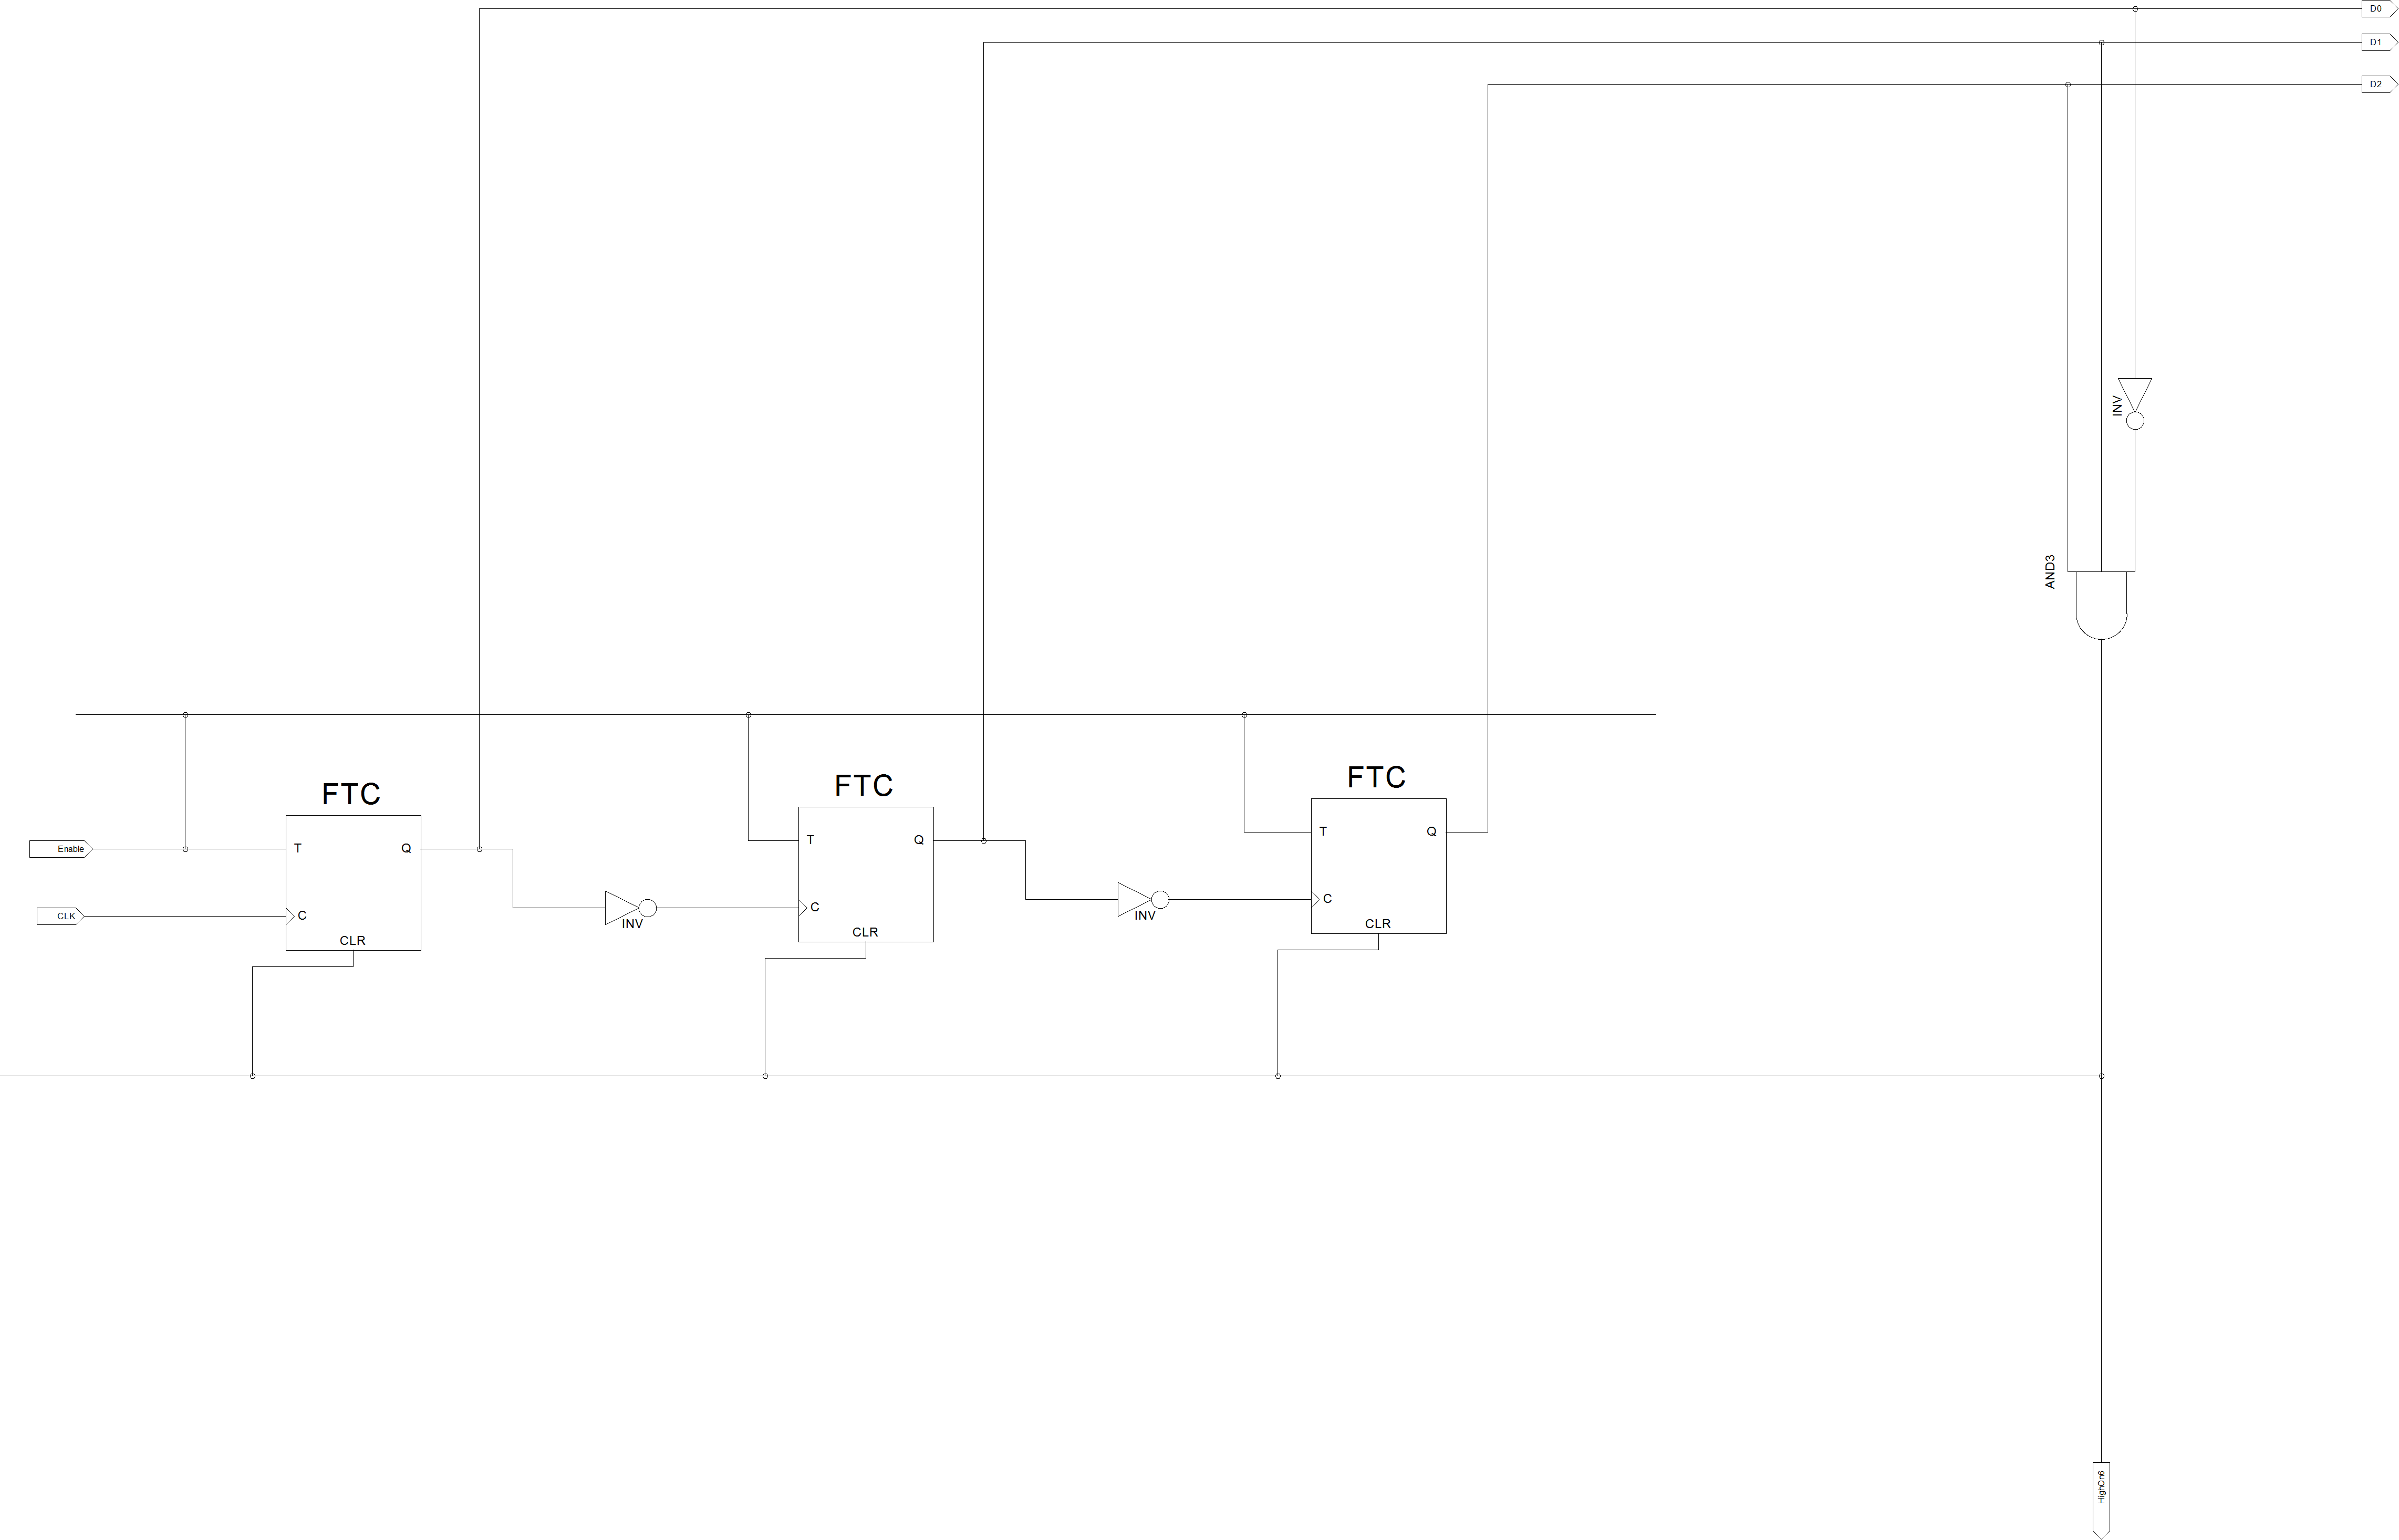
\includegraphics[width=\textwidth]{minute_6_counter.png}
             \end{center}
             
             \newpage
             \textbf{Symbol.}
   
             \begin{center}
                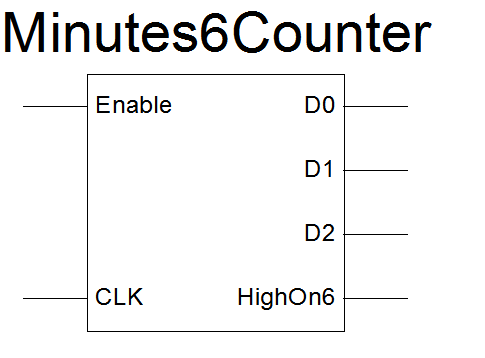
\includegraphics[width=\textwidth]{minute_6_counter_sym.png}
             \end{center}
             
             \textbf{Description.} The minute 6 counter is a 2-input to
             4-output counter. It counts from 0 - 5 and resets on 5. On each
             clock input, it increments by 1, and its current states are stored in
             the outputs D2, D1, and D0, listed from most significant
             bit to least significant bit. When the state is momentarily
             $110_2$ ($6_{10}$), the output HighOn6 goes high. This circuit will
             be used in the counting the minute tens.
             
  	\item[\textbf{Hour3Counter.}] \textbf{Schematic.}
   
             \begin{center}
                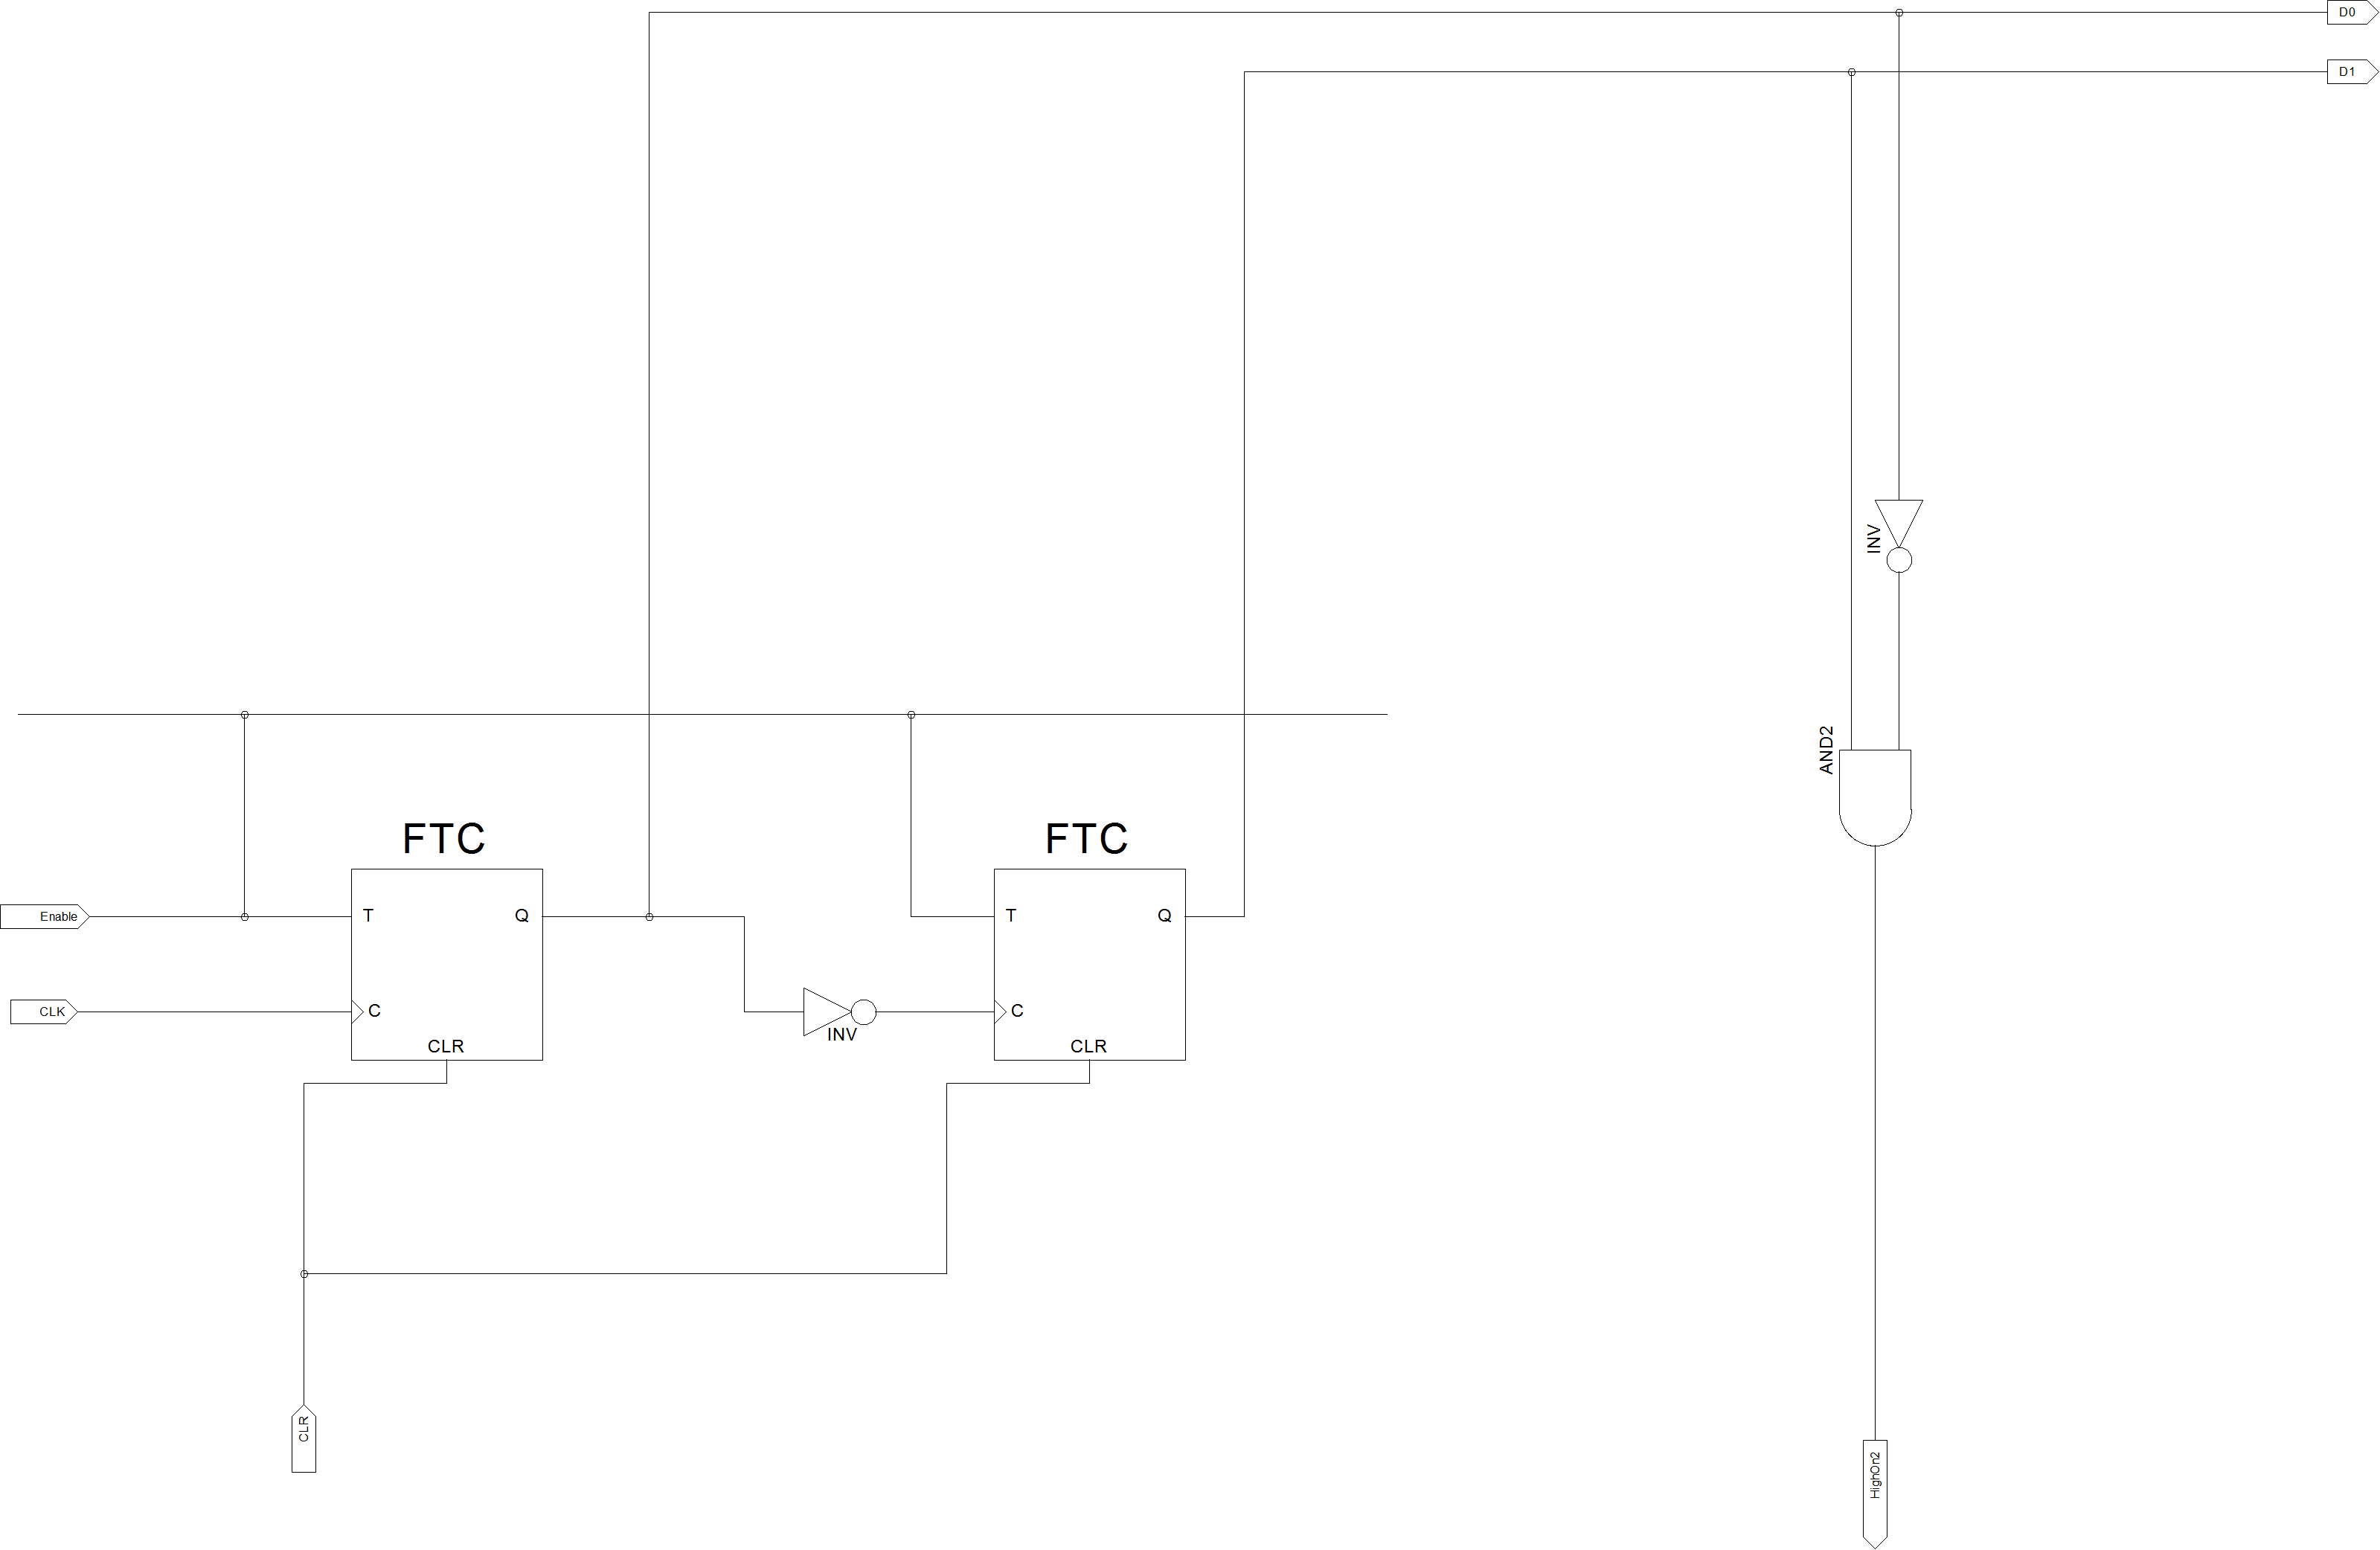
\includegraphics[width=\textwidth]{hour_3_counter.png}
             \end{center}
             
             \newpage
             \textbf{Symbol.}
   
             \begin{center}
                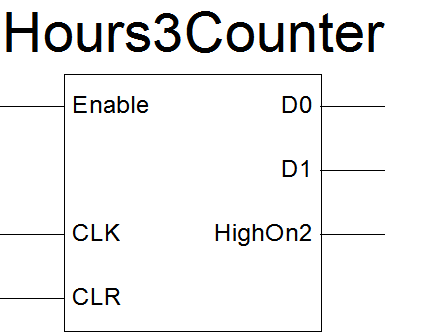
\includegraphics[width=\textwidth]{hour_3_counter_sym.png}
             \end{center}
             
             \textbf{Description.} The hour 6 counter is a 3-input to
             3-output counter.  On each clock input, it increments by 1, and its
             current states are stored in D1, and D0, listed from most significant
             bit to least significant bit.It is used for counting the hour tens.
             Unlike the other  counters above it does not automatically reset
             when it reaches 3. Instead we shall rely upon external circuit to
             reset this counter when the HighOn2 output(which goes high when
             D1 = 1 and D0 = 0) is high and when hour ones is HighOn4 (see
             decade counter plus above).
             
  	\item[\textbf{FourToSevenLEDs.}] \textbf{Schematic.}
   
             \begin{center}
                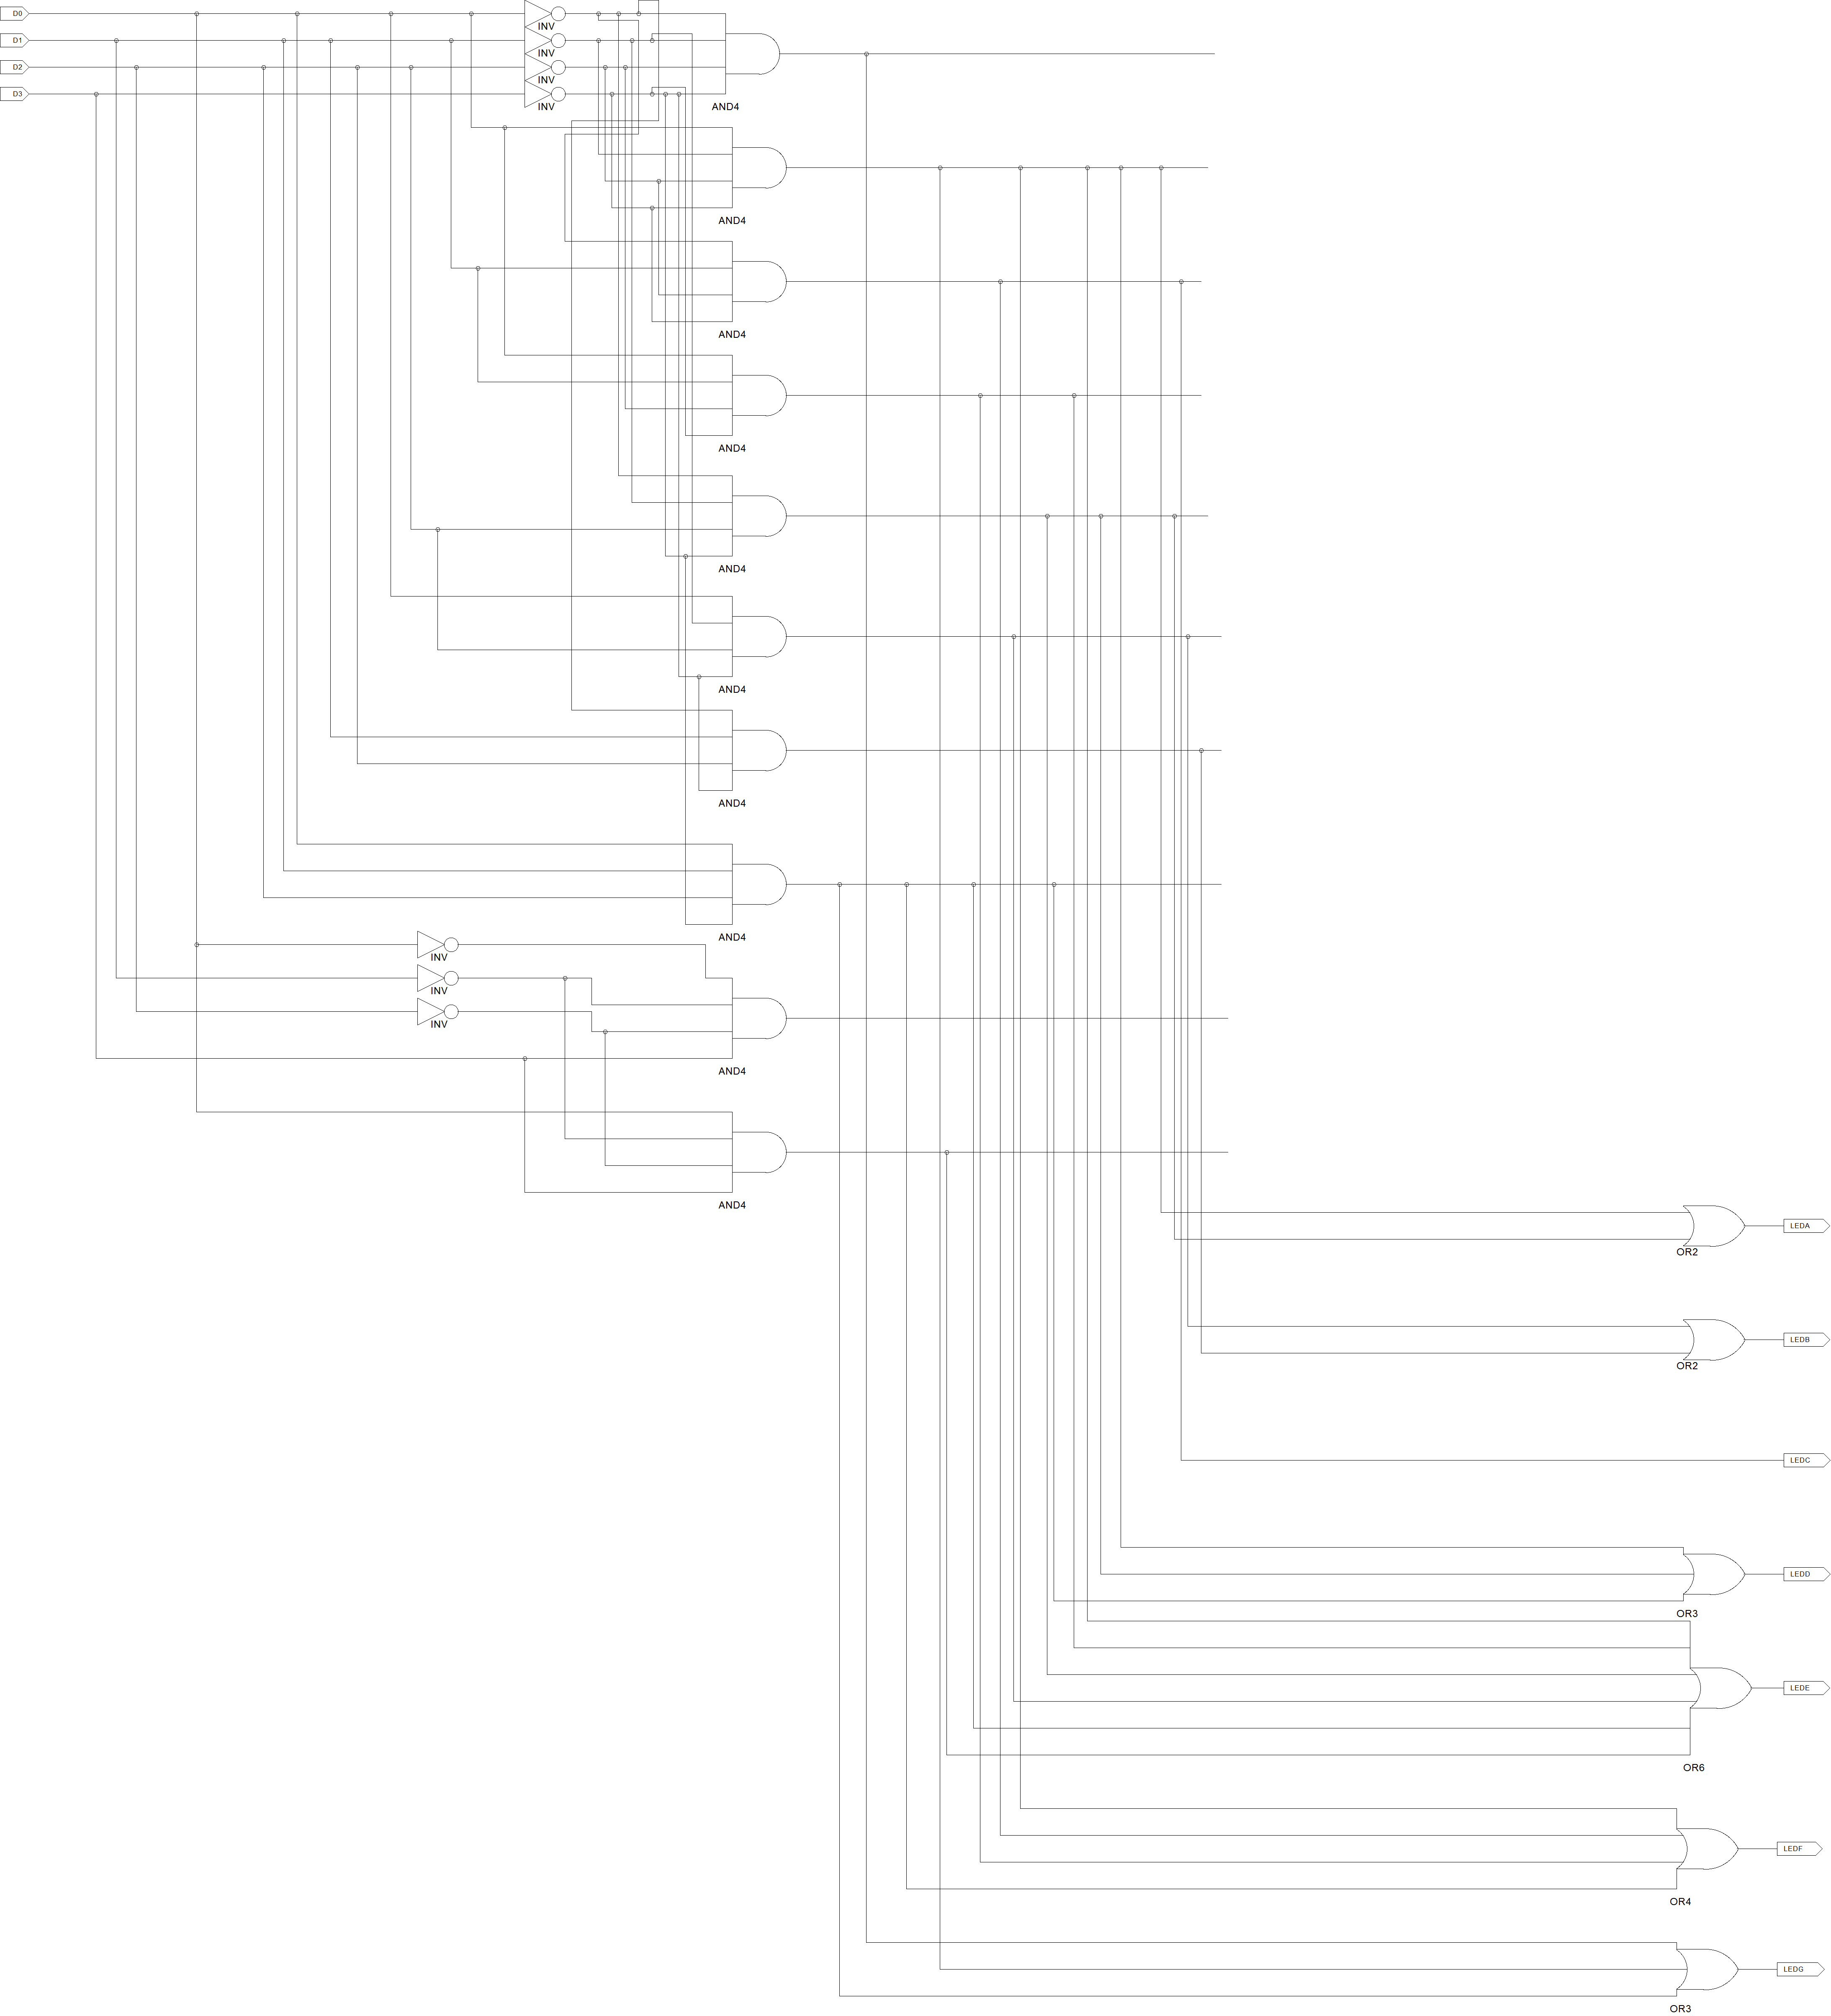
\includegraphics[width=\textwidth]{FourToSevenLEDs.png}
             \end{center}
             
             \newpage
             \textbf{Symbol.}
   
             \begin{center}
                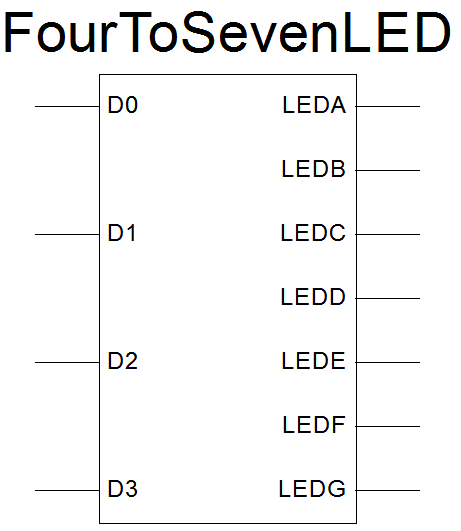
\includegraphics[width=\textwidth]{FourToSevenLEDsSym.png}
             \end{center}
             
             \textbf{Description.} This is a 4-input to 7-output circuit used
             for displaying decimal numbers (0-9) on a LED segment. The four
             bit input(D3, D2, D1, D0), where D0 is the least significant bit,
             is simply displayed on the 7 Segment LEDs.
             
  	\item[\textbf{ClockFreqDividerPlus.}] \textbf{Schematic.}
   
             \begin{center}
                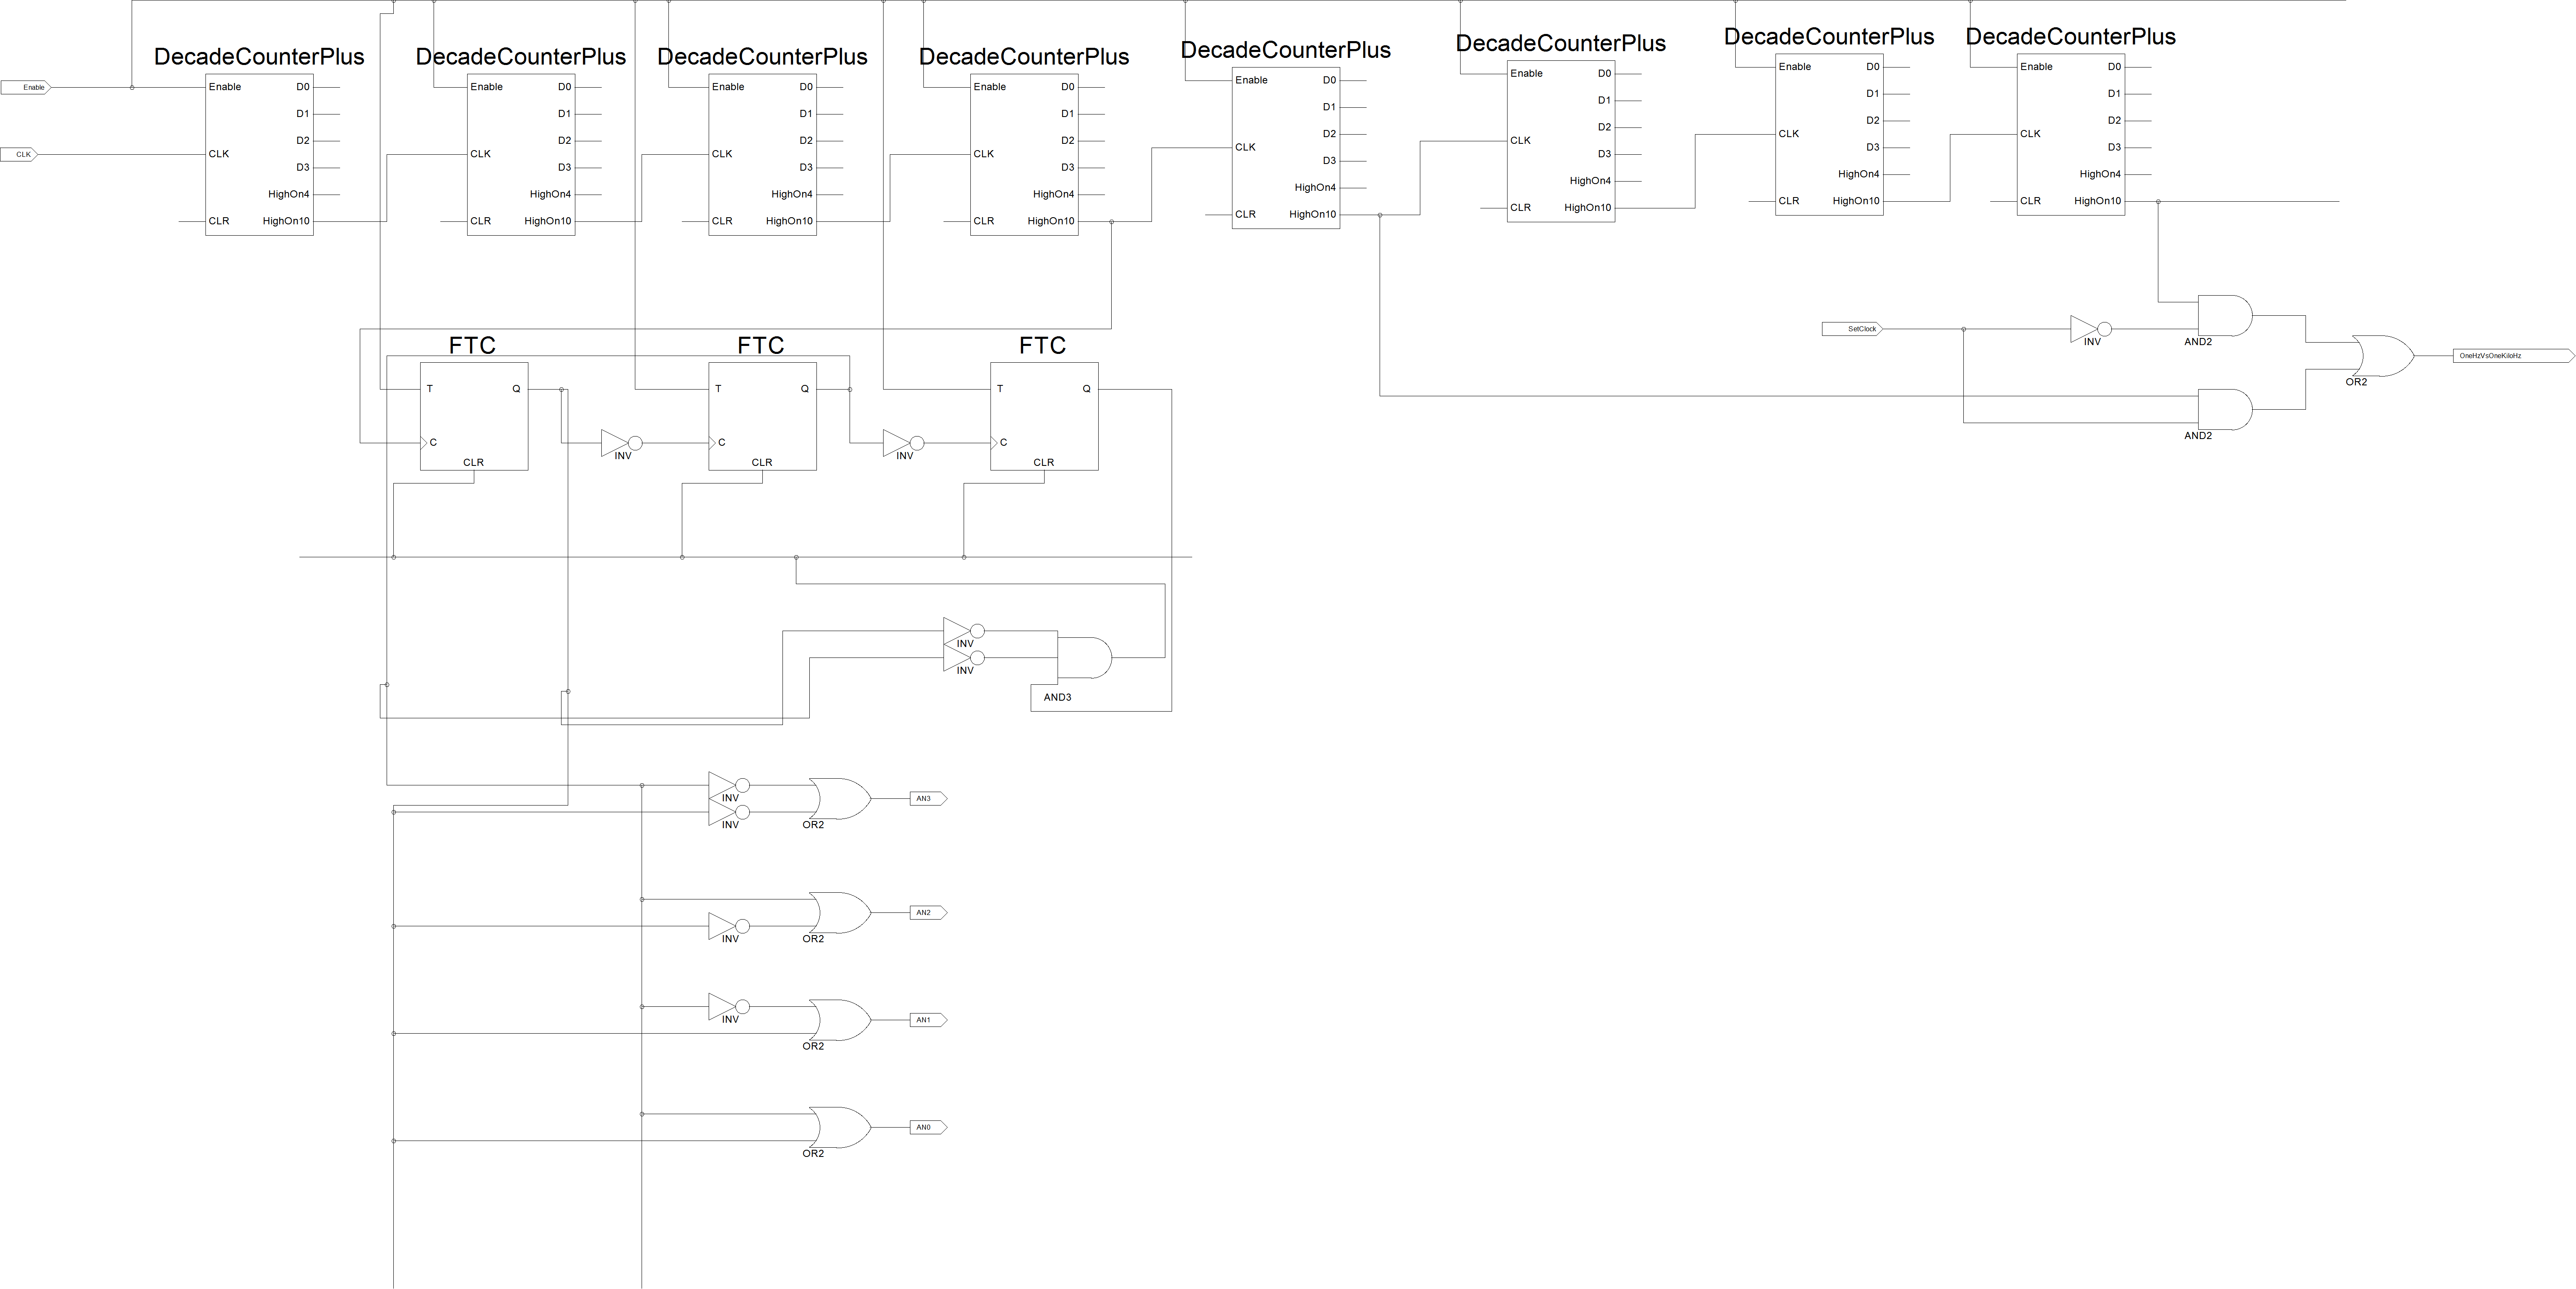
\includegraphics[width=\textwidth]{ClockFreqDivider.png}
             \end{center}
             
             \newpage
             \textbf{Symbol.}
   
             \begin{center}
                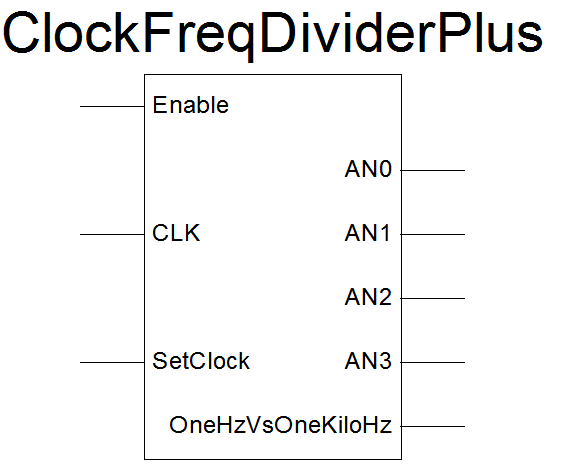
\includegraphics[width=\textwidth]{ClockFreqDividerSym.png}
             \end{center}
             
             \textbf{Description.} This circuit divides the 100MHz Clock
             frequency on our board to 1Hz. Thus it is a clock frequency
             divider. The set clock input blocks the 1Hz output and instead
             allows a 1000Hz to go through. The AN0, AN1, AN2, and AN3 outputs
             are used to select a particular 7-segment LED to display. We used
             a 2-4 decoder to periodically select exactly one of AN0, AN1, AN2,
             and AN3. The inputs to the decoder are taken from the state of a
             counter (clocked by selecting the input of the 10000Hz Flip Flop
             (see schematic)). By periodically selecting a particular 7-segment,
             we create an illusion that all segments are always on. This method
             works because the human eye cannot detect such a fast frequency.
             Note that the output of the decoder are inverted because a 7-segment
             is active low.
             
  	\item[\textbf{Digital Clock.}] \textbf{Schematic.}
   
             \begin{center}
                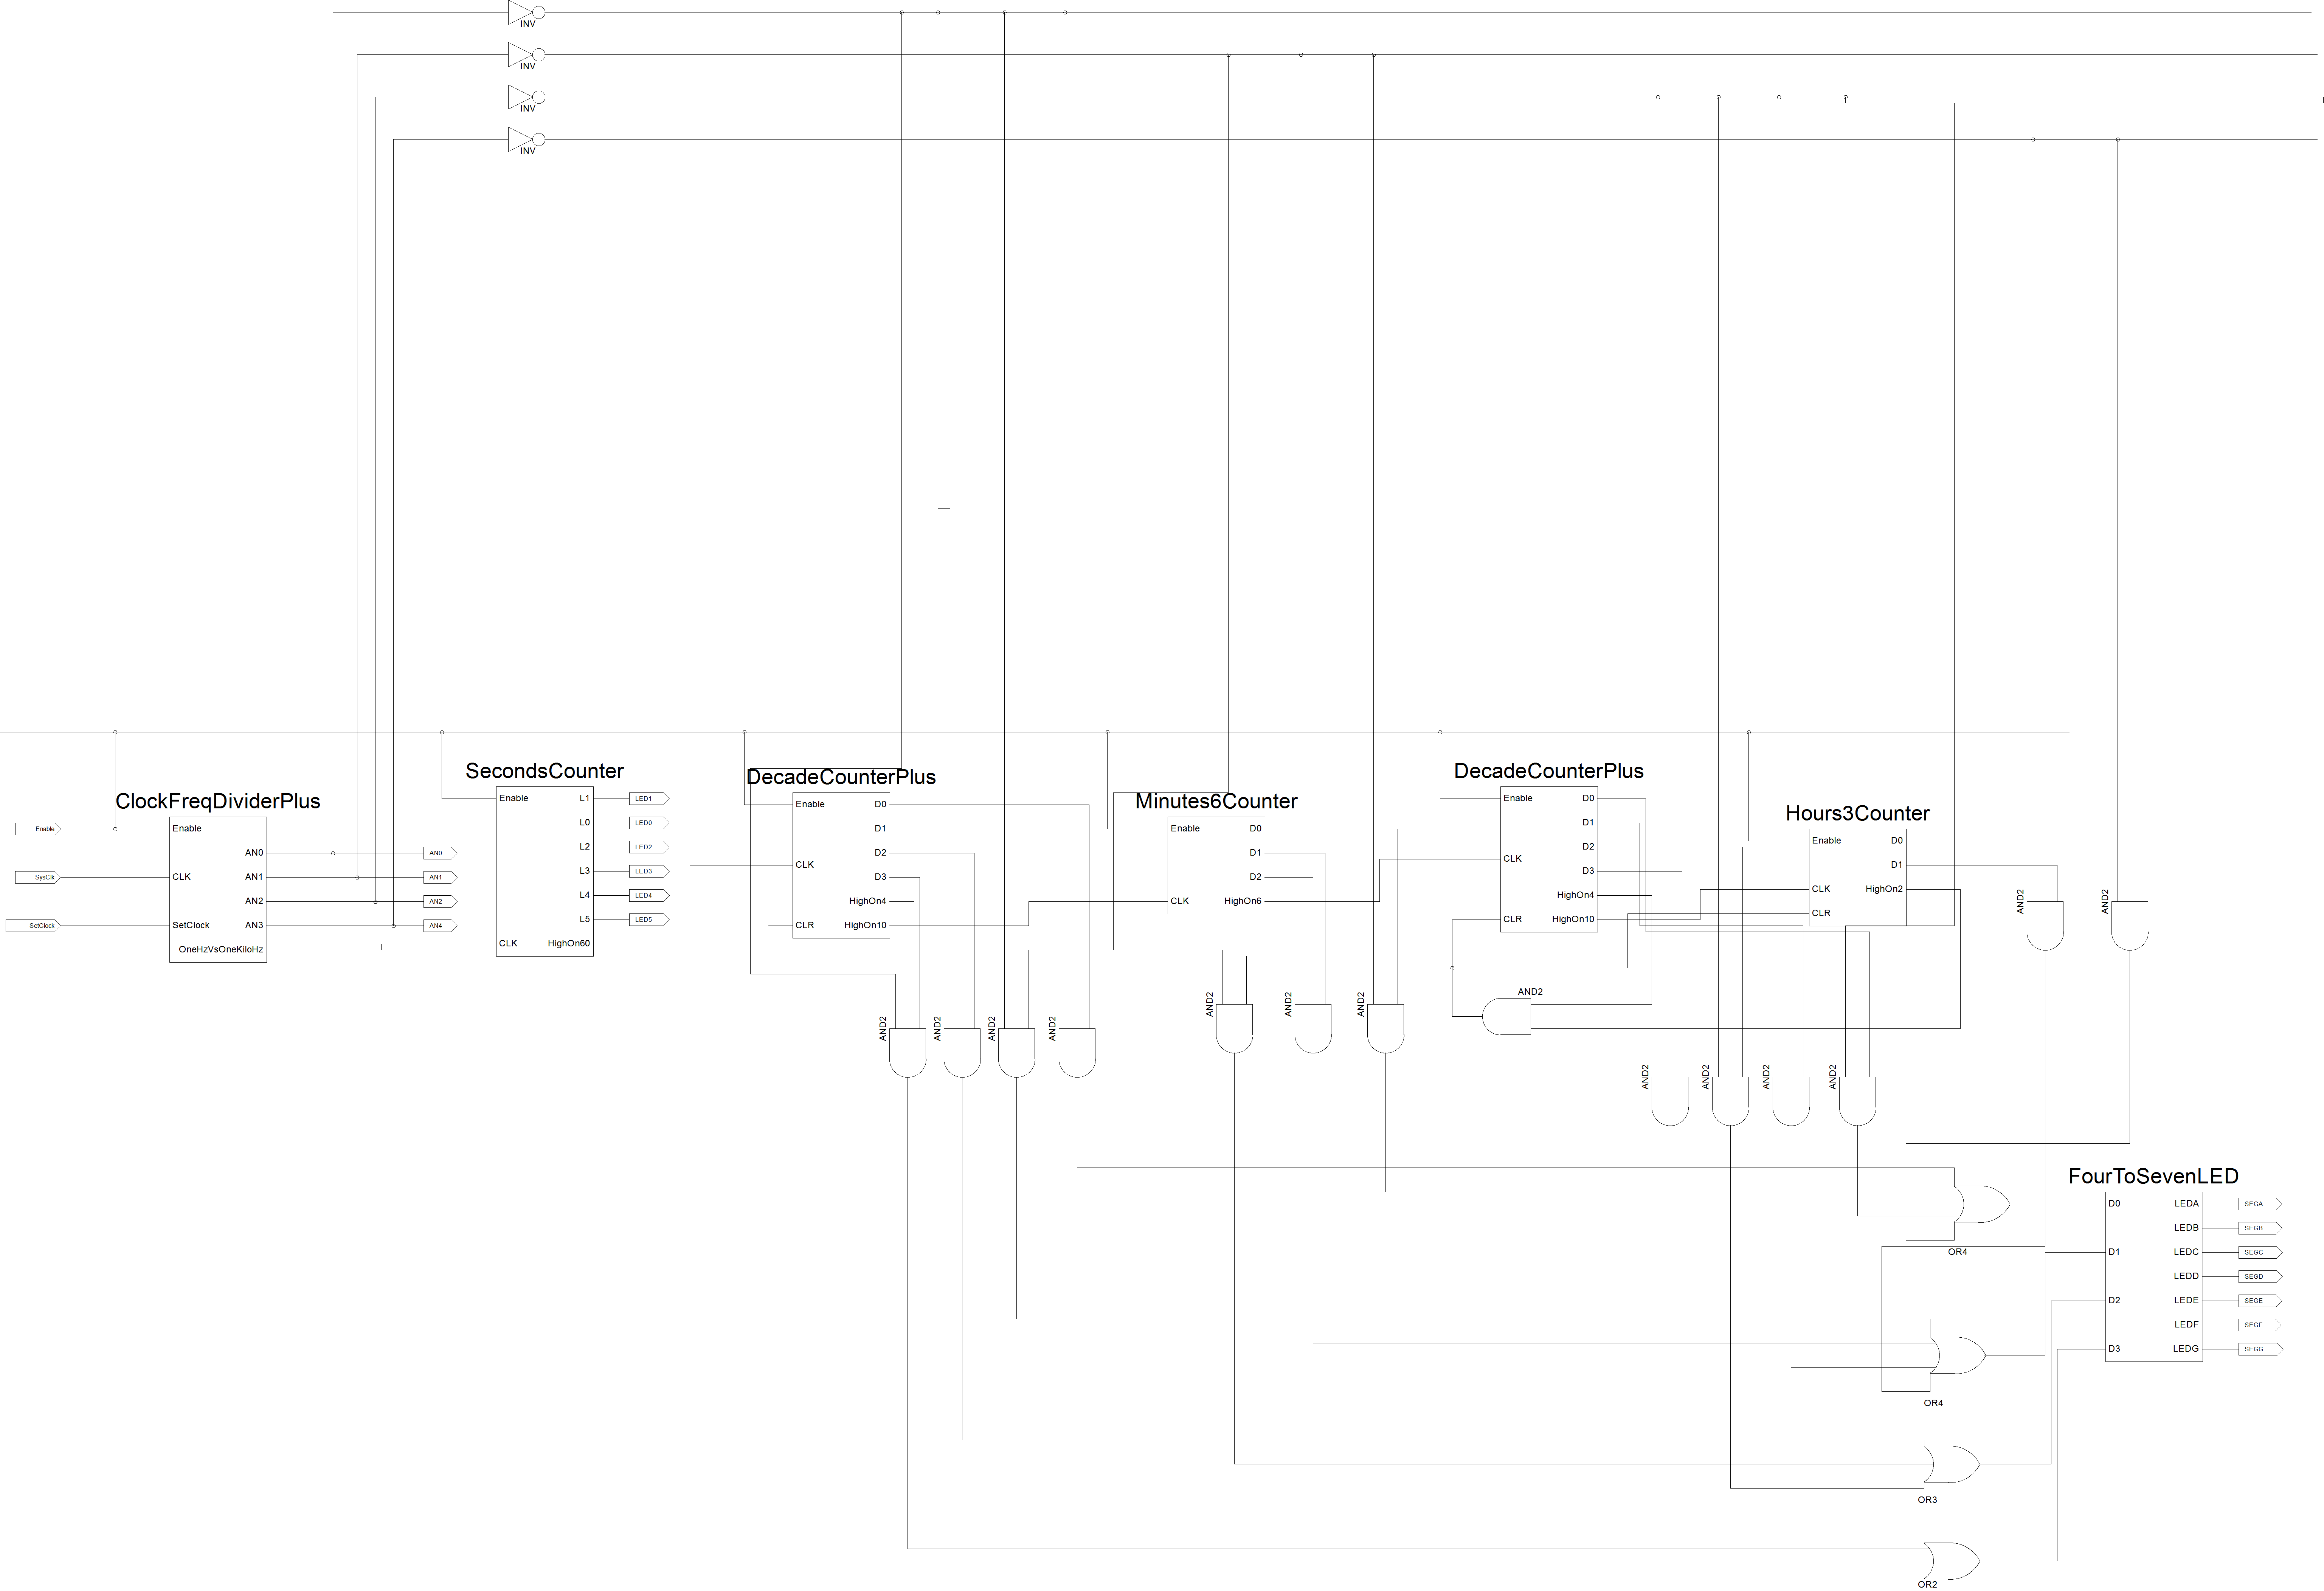
\includegraphics[width=\textwidth]{Driver.png}
             \end{center}
             
             \newpage
             \textbf{Symbol.}
             
             \textbf{Description.} Now we put everything together to create our
             digital clock. The clock on the board will clock the frequency
             divider; then the frequency divider will clock the seconds counter;
             the seconds counter will clock the minute ones; the minute ones
             will clock the minute tens; the minute tens will clock the hour
             ones; and the hour ones will clock the hour tens; we also tie all
             the output of the decimal outputs using OR gates to the corresponding
             inputs of the 4-7 display. 
   
   
   
\end{enumerate}
\end{document}
